As \acrshort{ux} design is its own extensive field of research and visualisations were a secondary aim, we took inspiration from existing well designed visualisers TensorFlow Playground and Algorithm Visualizer.

%TC:ignore
\begin{figure}[H]
    \begin{minipage}{0.54\textwidth}
        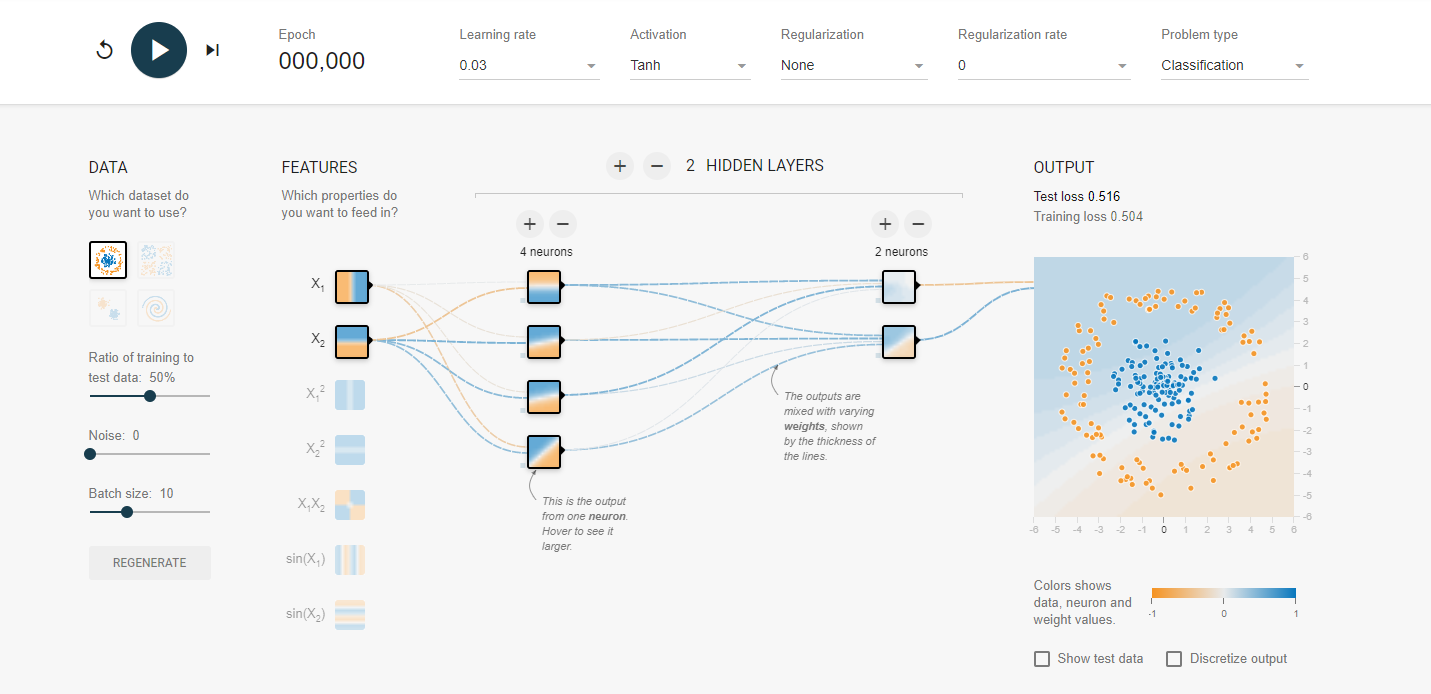
\includegraphics[height=4.3cm]{images/tensor-flow-playground.png}
        \caption{TensorFlow Playground\\\url{https://playground.tensorflow.org/}}
        \label{fig:tensorflow_playground}
    \end{minipage}
    \begin{minipage}{0.46\textwidth}
        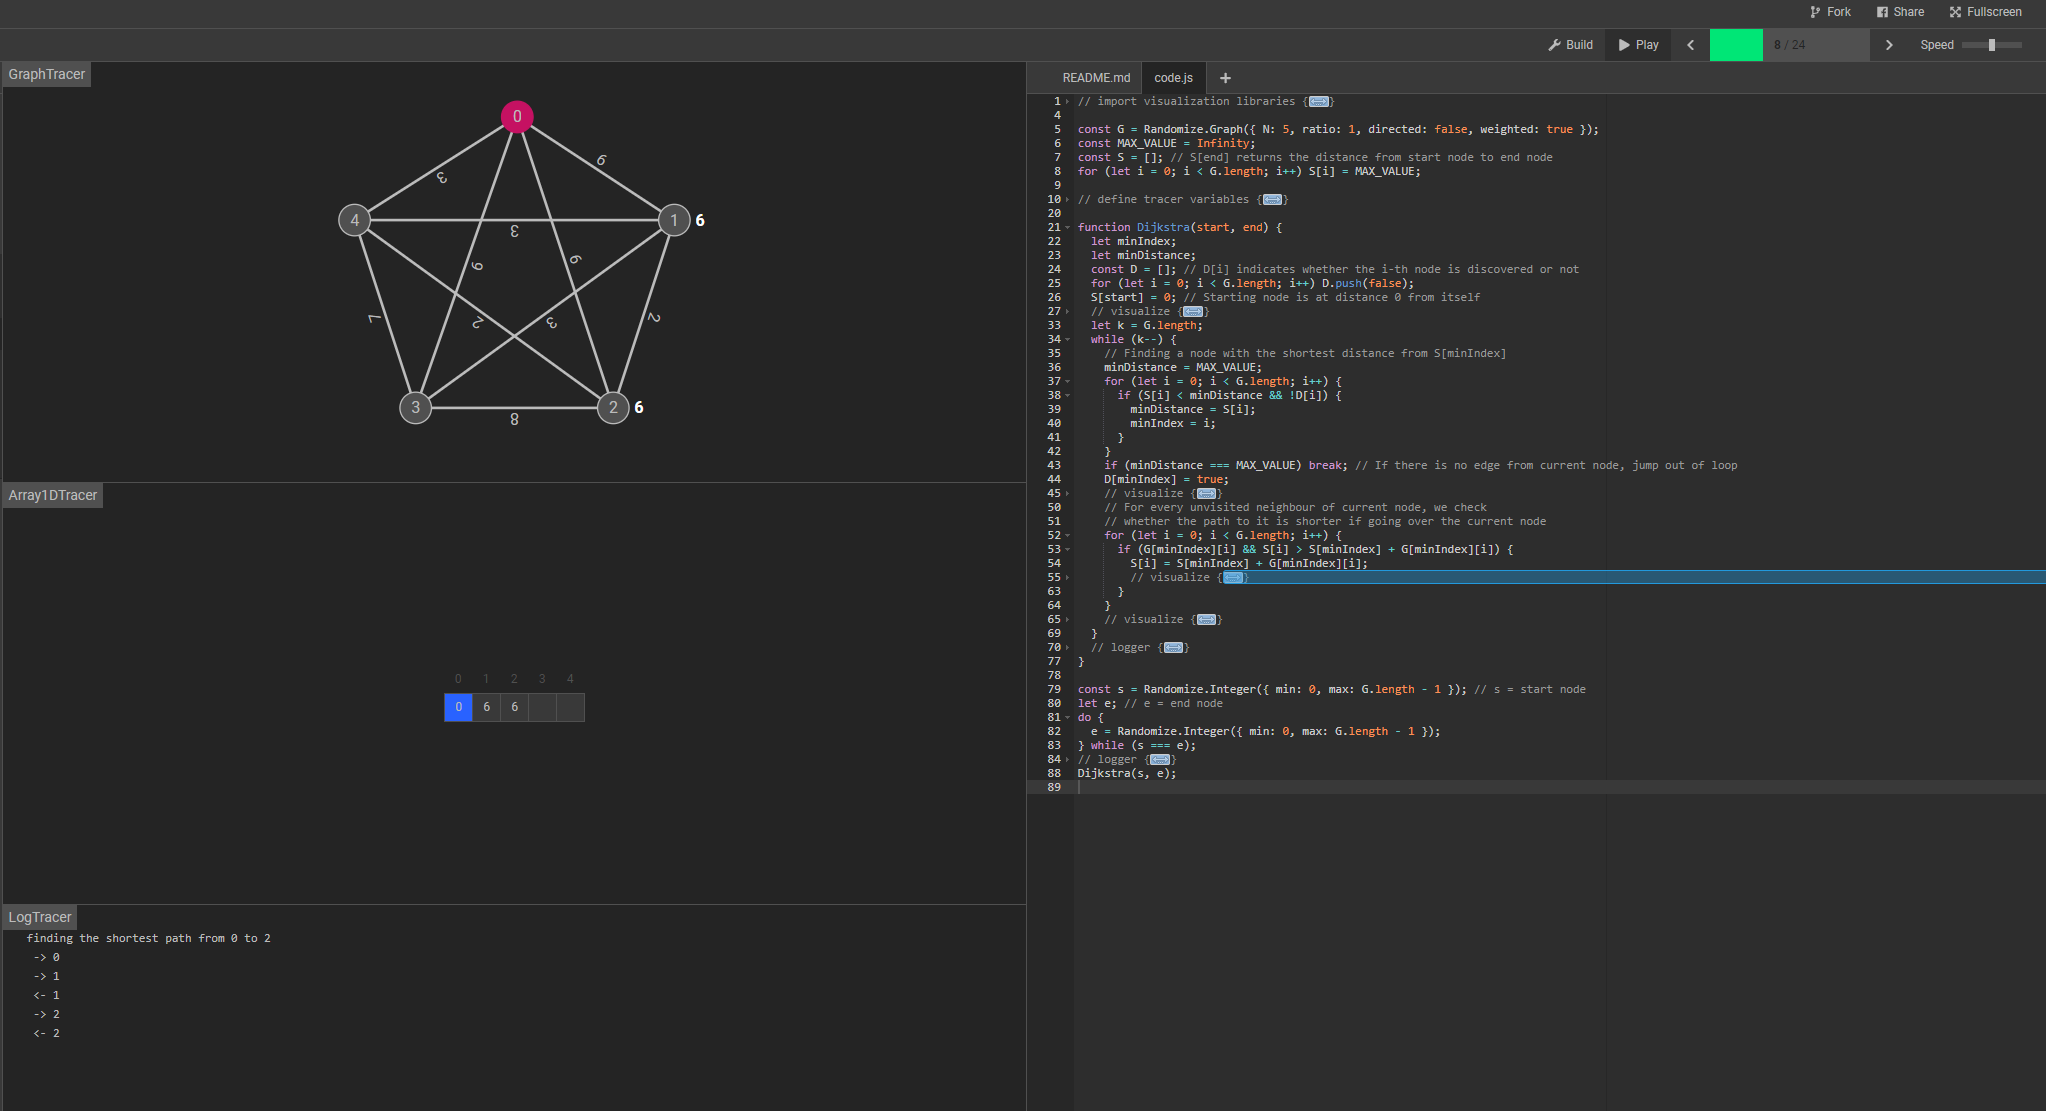
\includegraphics[height=4.3cm]{images/algorithm-visualizer.png}
        \caption{Algorithm Visualizer\\\url{
https://algorithm-visualizer.org/}}
        \label{fig:algorithm_visualizer}
    \end{minipage}
\end{figure}
%TC:endignore

The key features that make both of them effective are separated panels for configuration, graphs and information. Furthermore TensorFlow playground has tooltips giving information for unlabeled components. Algorithm Visualizer allows the user to step back and forth between an algorithm. They both have a degree of interactivity, allowing users to change the input parameters to the problem.

To keep our functionality focused, we decided to separate the solution visualisation (\cref{section:solution_visualisation}) and interactive algorithm visualisation (\cref{section:stepped_visualisation}) components into separate pages.